\graphicspath{{Annexes/}}
\appendix


\chapter{Code traitement des intents}
\label{Code}

\begin{figure}[h]
	\centering
		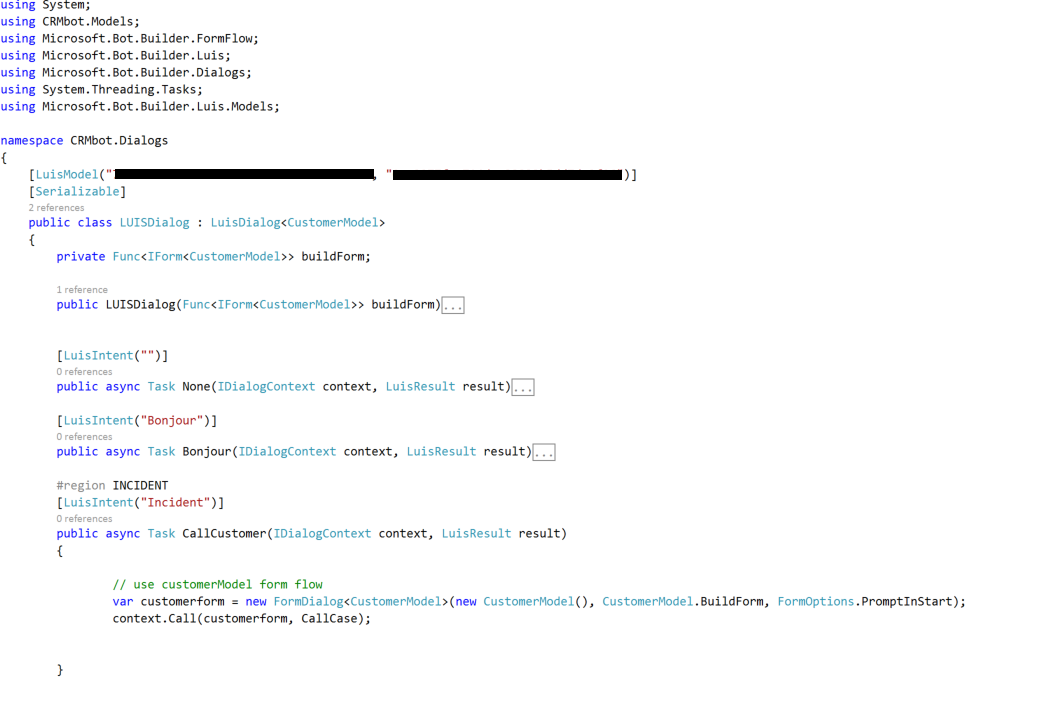
\includegraphics[width = \textwidth]{code.png}
\end{figure}


\chapter{Dialogue avec le chatbot}
\label{Dialogue chatbot}

Début du dialogue, intent bonjour, intent incident et demande du numéro client :
\vspace{1em}

\begin{figure}[ht]
	\centering
		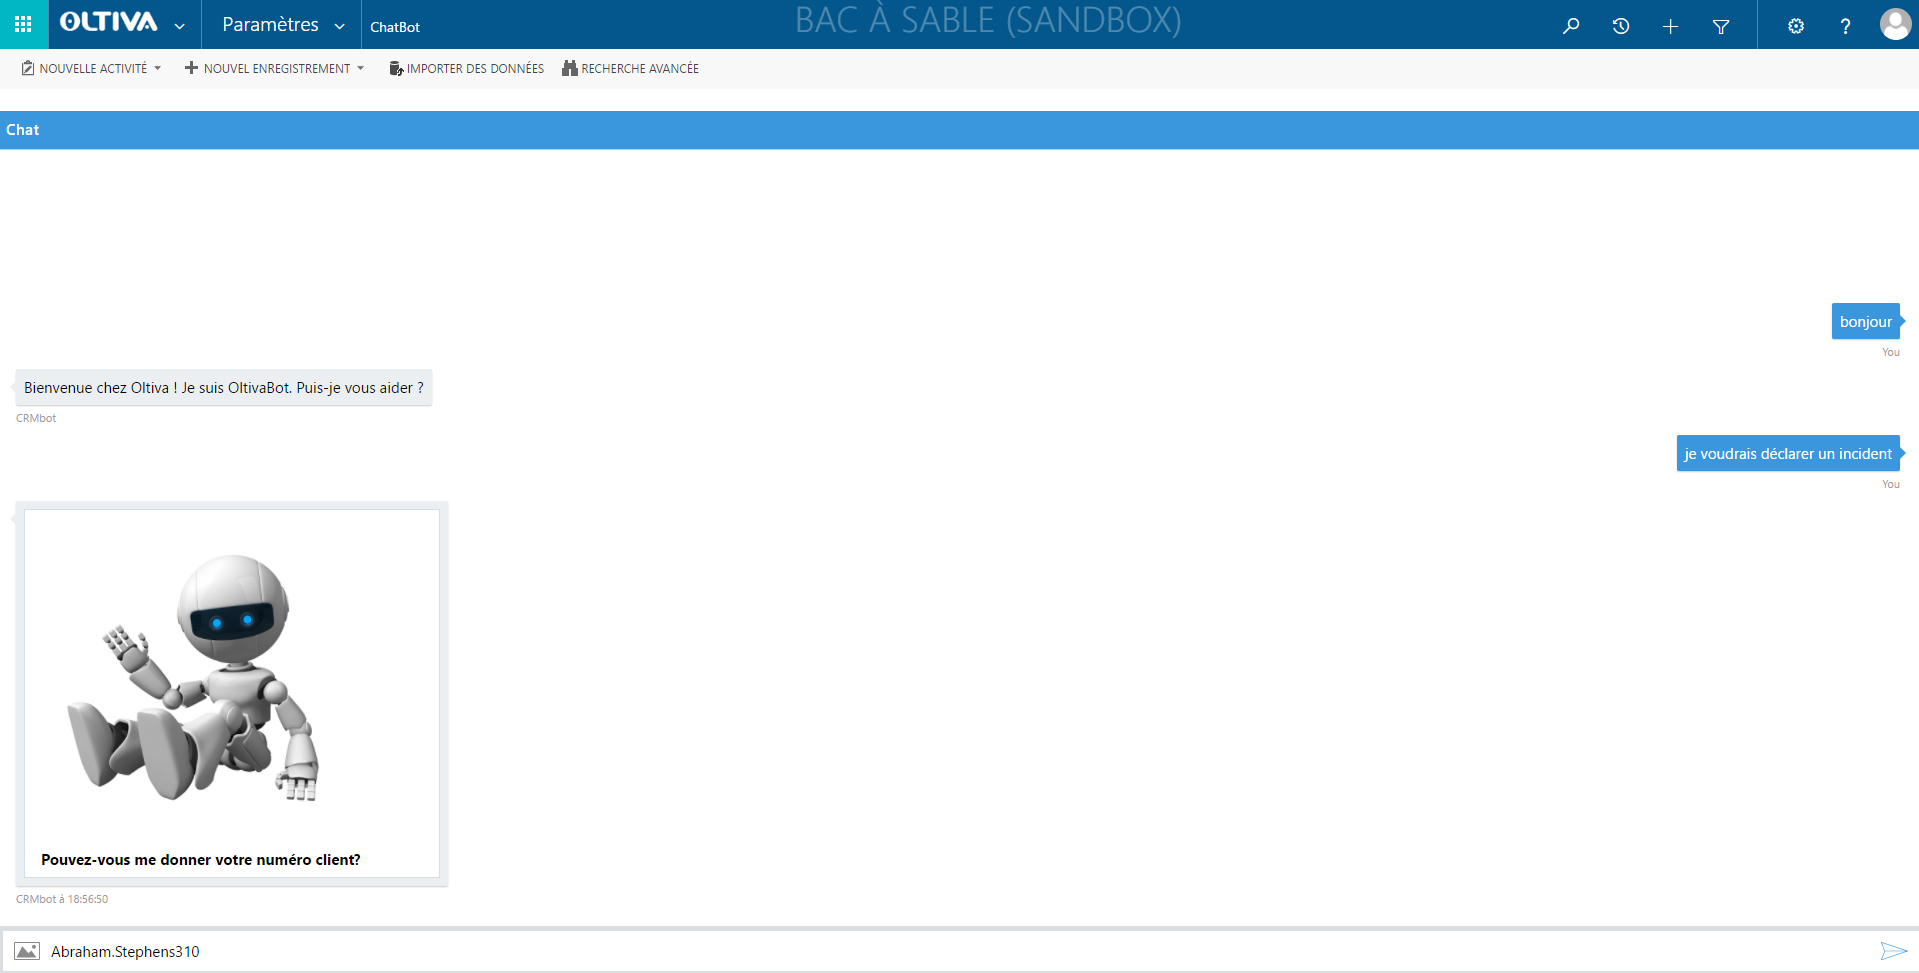
\includegraphics[width = 0.8\textwidth]{1.png}
\end{figure}

Choix de l’incident :
\vspace{1em}

\begin{figure}[ht]
	\centering
		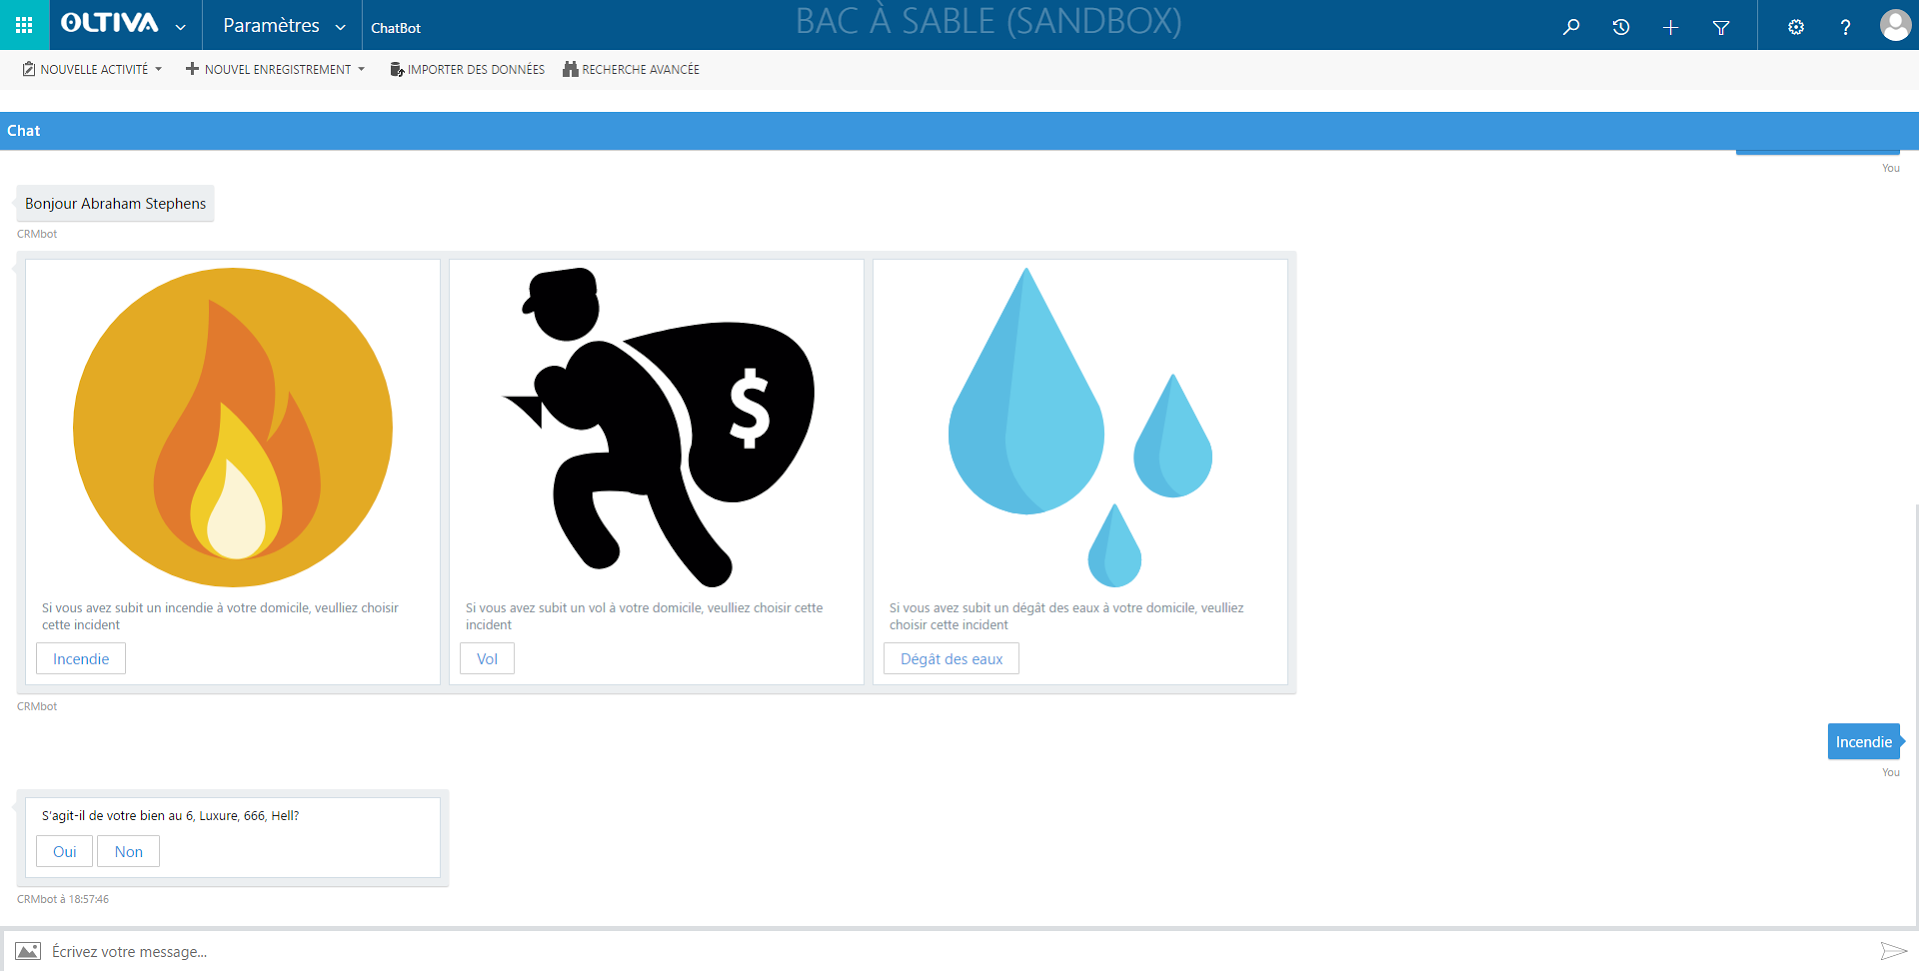
\includegraphics[width = 0.8\textwidth]{2.png}
\end{figure}

Confirmation de l’adresse, fausse donc demande des informations :
\vspace{1em}

\begin{figure}[ht]
	\centering
		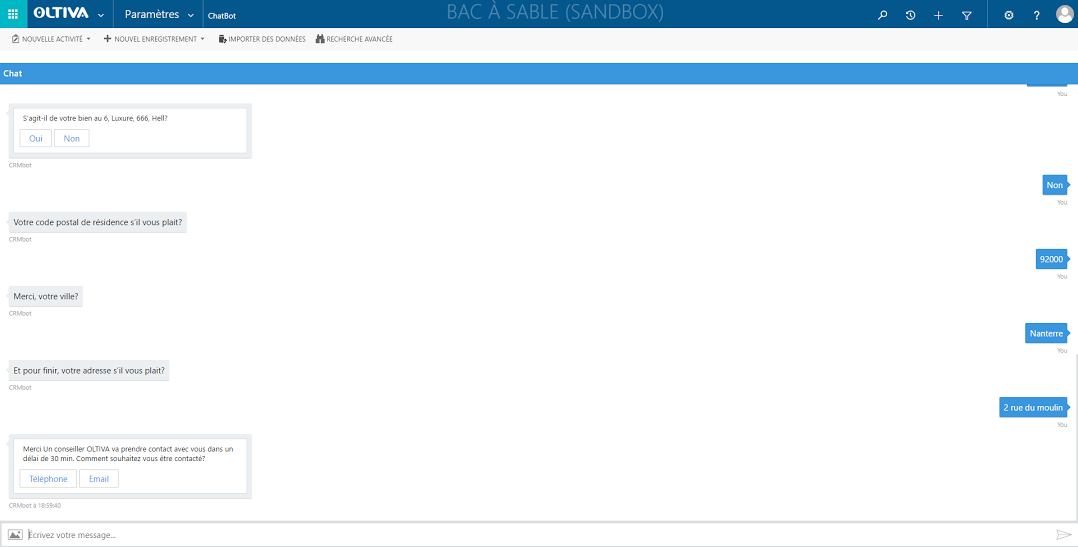
\includegraphics[width = 0.8\textwidth]{3.png}
\end{figure}


Choix de la manière d’être contacté, téléphone choisi donc confirmation du téléphone dans CRM. Pas d’autres questions donc fin de la conversation.
\vspace{1em}

\begin{figure}[ht]
	\centering
		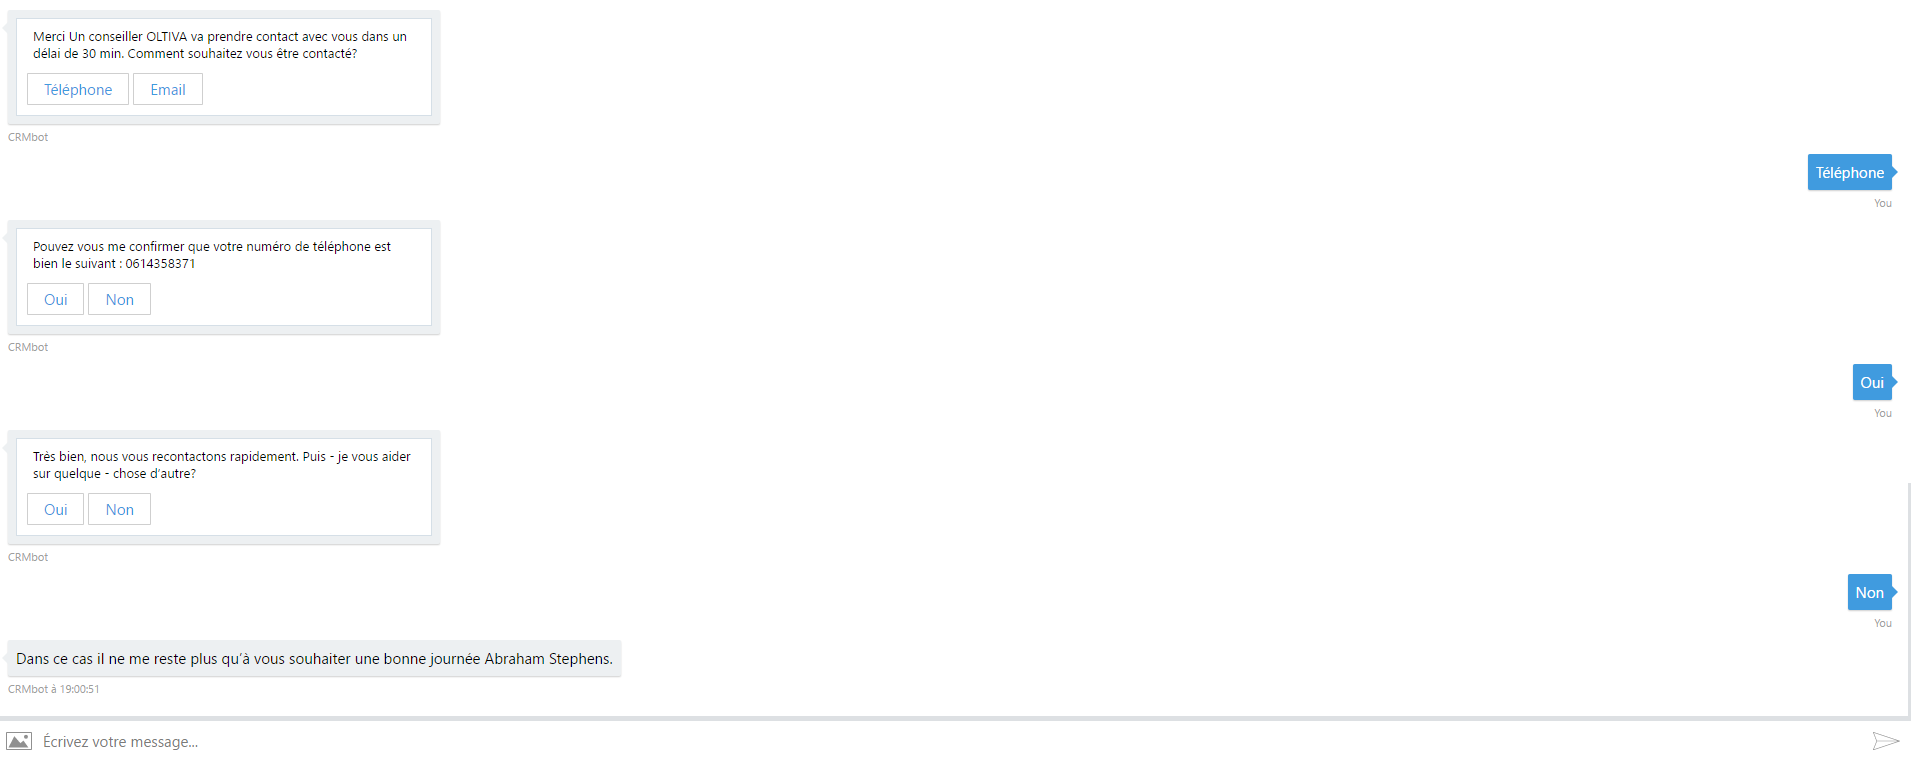
\includegraphics[width = 0.8\textwidth]{finConv.png}
\end{figure}